\begin{figure}[h]
    \centering
    \setlength{\resLen}{1.in}
    \addtolength{\tabcolsep}{-3pt}
    \small
    \begin{tabular}{cccccc}
        
\includegraphics[height=\resLen]{waveoptics/slab/N1_300nm.jpg} &
        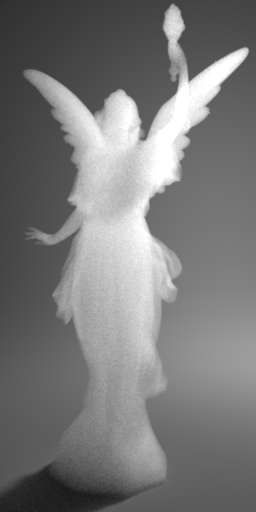
\includegraphics[height=\resLen]{waveoptics/slab/N100_300nm.jpg} &
        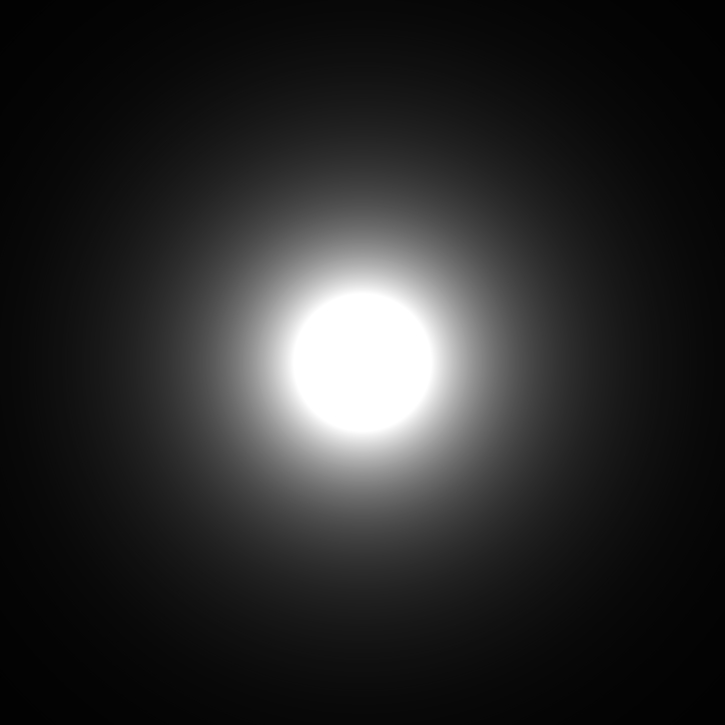
\includegraphics[height=\resLen]{waveoptics/slab/N100_500nm.jpg} &
        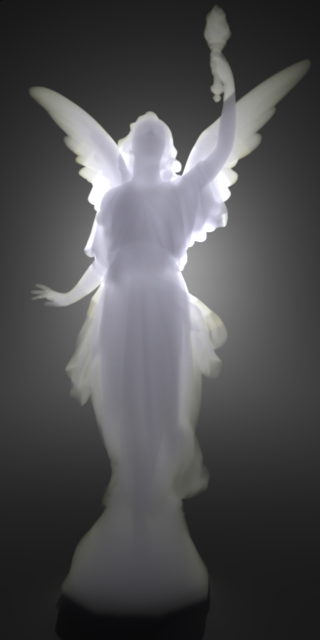
\includegraphics[height=\resLen]{waveoptics/slab/color.jpg} & 
        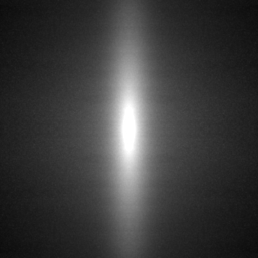
\includegraphics[height=\resLen]{waveoptics/slab/aniso_y.jpg} &
        \includegraphics[height=\resLen]{waveoptics/slab/pos.jpg}
        \\
        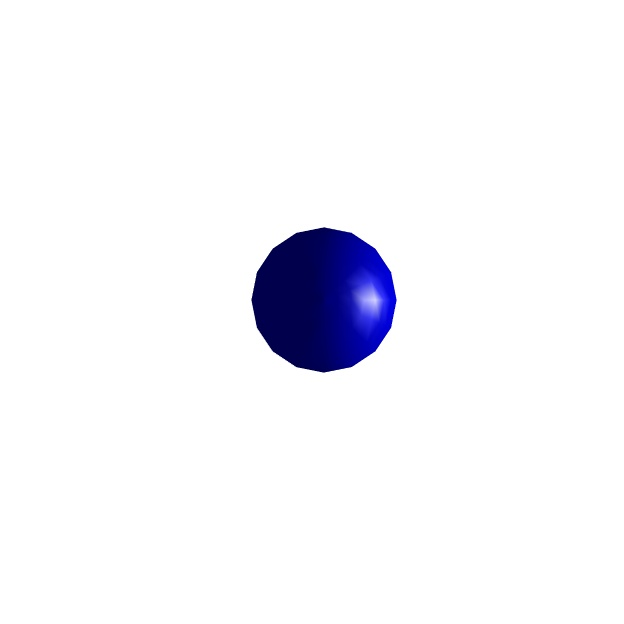
\includegraphics[height=\resLen]{waveoptics/particle/300nm_N1.jpg} &
        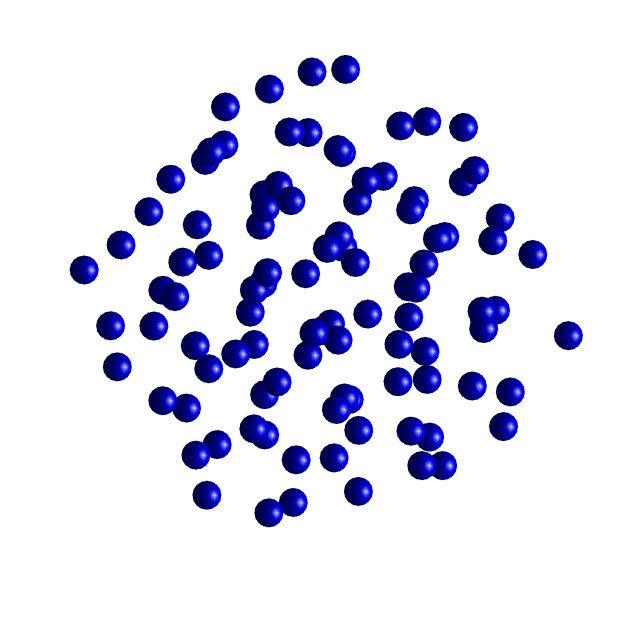
\includegraphics[height=\resLen]{waveoptics/particle/300nm_N100.jpg} &
        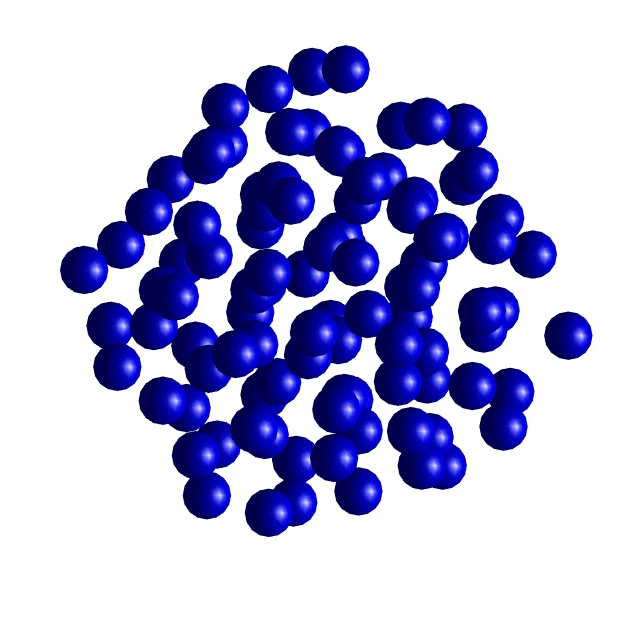
\includegraphics[height=\resLen]{waveoptics/particle/500nm_N100.jpg} &
        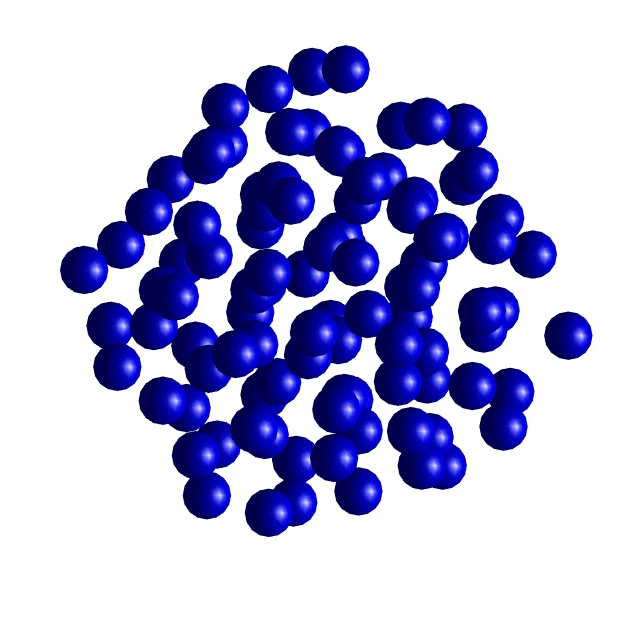
\includegraphics[height=\resLen]{waveoptics/particle/500nm_N100.jpg} &
        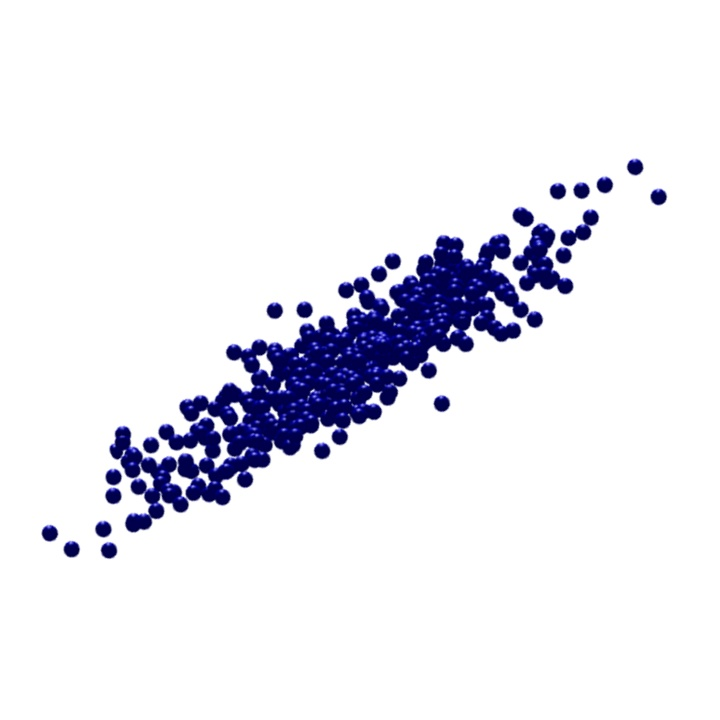
\includegraphics[height=\resLen]{waveoptics/particle/aniso.jpg} &
        \includegraphics[height=\resLen]{waveoptics/particle/pos.jpg}
        \\
        $\Ncls=1$   &
        $\Ncls=100$ &
        $\Ncls=100$ &
        $\Ncls=100$ & 
        $\Ncls=100$ &
        $\Ncls=100$
        \\
        $\radius_i=300\text{nm}$ &
		$\radius_i=300\text{nm}$ &
		$\radius_i=500\text{nm}$ &
		$\radius_i=500\text{nm}$ & 
		$\radius_i=500\text{nm}$ &
		$\radius_i=500\text{nm}$
		\\
        Isotropic & Isotropic & Isotropic & Isotropic & Anisotropic & Pos. correlated
        \\
        $\lambda=700\text{nm}$ &
        $\lambda=700\text{nm}$ &
        $\lambda=700\text{nm}$ &
        Multi-spectral &
        $\lambda=700\text{nm}$ &
        $\lambda=400\text{nm}$
    \end{tabular}
    \caption[Teaser]{\label{fig:waveoptics:teaser}
        We introduce a new technique to compute bulk scattering parameters (i.e., the extinction and scattering coefficients as well as the single-scattering phase function) in a systematic fashion. By considering wave optical effects and particle (scatterer) interactions at the microscopic level, our technique enjoys the generality of supporting a wide range of media (e.g., isotropic, anisotropic, and correlated).
        In this figure, we show renderings of thin slabs lit with a small area light from behind (top).
        Additionally, we show visualizations of the corresponding particle distributions (middle) as well as per-cluster particle counts~$\Ncls$ radii $\radius_i$ (bottom).
    }
\end{figure}
